\documentclass[column,brazilian,12pt,a4paper,final]{article}
\usepackage[brazil]{babel}
%\usepackage{nonfloat}
\usepackage[utf8]{inputenc}
\usepackage{multicol}
\usepackage{hyperref}
\usepackage[pdftex]{color,graphicx}
\usepackage{geometry}
\usepackage{amsmath}
\usepackage{caption}

 \geometry{
 a4paper,
 total={170mm,257mm},
 left=20mm,
 top=20mm,
 }
 \usepackage{ragged2e}
\usepackage{fancyhdr}
\usepackage{caption}[=v1]
\usepackage{xcolor}
\usepackage{circuitikz}
\pagestyle{plain}
\fancyhead{}
\lhead{
\includegraphics[width=1.5cm]{logoufrgs}}
\rhead{
\includegraphics[width=0.8cm]{logoif}}
\fancyfoot{}
\fancyhead[C]{\footnotesize Física Experimental III $\bullet$ 2025/1}
\fancyfoot[RO]{\thepage}
\usepackage{float}
\usepackage{setspace}
\usepackage{fancyref}


\title{Lei de Faraday-Lenz: Verificação Experimental e Cálculo da Constante de Permeabilidade Magnética do Ferro}
\author{Autores: \\ Lucas Assis Paulino da Silva - 590174 \\Lucas Bertazo de Deus Félix - 587064
 \\ Pedro Henrique Reis de Oliveira - 590908 \\ IF-UFRGS}
\date{Junho 2025}

\begin{document}
\maketitle
\thispagestyle{fancy}

\section*{Resumo}
\paragraph{}
Neste trabalho, investigamos o fenômeno da indução eletromagnética, validando experimentalmente a Lei de Faraday-Lenz. Utilizando um arranjo com uma bobina geradora (1.000 espiras), uma bobina detectora (10.000 espiras) e um osciloscópio, medimos a força eletromotriz induzida em três cenários: com um ímã permanente, com a bobina geradora (eletroímã) e com a bobina geradora contendo um núcleo de ferro. A análise dos dados, realizada pela integração numérica da tensão induzida, permitiu o cálculo do fluxo magnético e do campo magnético para cada caso. A partir dos campos magnéticos do eletroímã com e sem o núcleo ($B_{\text{Nucleo}} = 2,24 \times 10^{-4}$ T e $B_{\text{Sem Nucleo}} = 1,08 \times 10^{-5}$ T, respectivamente) , determinamos a permeabilidade magnética do ferro como sendo $\mu = (2,60 \times 10^{-5} \pm 4,71 \times 10^{-7}) \frac{\text{T.m}}{\text{A}}$. Os resultados confirmaram a consistência da Lei de Faraday, com baixo desvio padrão nas medições de fluxo , e o valor de $\mu$ se mostrou coerente com o esperado para materiais ferromagnéticos.

\section{Introdução}
\paragraph{}
Um dos grandes eventos do século XIX para a ciência foi a descoberta do fenômeno da indução eletromagnética que permitiu a criação de uma ponte entre o magnetismo e a eletricidade. O físico britânico Michael Faraday foi responsável por deduzir experimentalmente a força eletromotriz induzida como sendo proporcional à taxa de variação de fluxo magnético sobre a área delimitada por um circuito.

Outros cientistas importantes como Lenz e James C. Maxwell foram cruciais para avanço teórico e o refinamento matemático das deduções advindas dos laboratórios. Lenz afirmou a inversão  no sentido da corrente induzida trazendo à tona o princípio da conservação de energia, por exemplo. Assim,os estudos referentes ao eletromagnetismo continuam a evoluir até os dias de hoje.

Este relatório, por sua vez, tem como objetivo a verificação prática destas leis por meio de experimentos que utilizarão de bobinas, circuitos e um osciloscópio como será melhor descrito nas sessões seguintes. Não somente permitindo uma melhor visualização dos fenômenos teoricamente estudados mas também possibilitando a exploração das variáveis fundamentais para a análise eletromagnética. 

\section{Embasamento Teórico}
\paragraph{}
Nesta seção, serão apresentados os fundamentos teóricos que governam os fenômenos de indução eletromagnética investigados. Iniciaremos com a dedução da equação para o campo magnético gerado por um solenoide a partir da Lei de Ampère , seguida pela formulação da Lei de Indução de Faraday-Lenz, que é central para a análise dos dados experimentais.
\subsection{Campo magnético produzido por um solenóide}
      Usando a \textit{lei de Ampère}:
      \begin{equation}
        \oint B \cdot d\ell = \mu_0 I_{int}
      \end{equation}
      Onde $B$ é o campo magnético, $d\ell$ é um elemento 
      infinitesimal da 
      curva $C$, $\mu_0$ é a constante de permeabilidade magnética 
      do vácuo
      e $I_{int}$ é a corrente interna à curva $C$.
      \\\\
      Implementando uma curva amperiana $C$ retangular delimitada 
      pelos pontos 
      \{\textit{A, B, C, D}\}, dos quais \{\textit{A, B}\} estão no 
      interior do solenóide, de maneira que o campo magnético fique na 
      mesma 
      direção da curva, e \{\textit{C, D}\} são pontos externos a
      esse, onde não há campo:
      \begin{equation}
        \oint \vec{B} \cdot d\vec{\ell} = \int_a^b \vec{B} \cdot 
        d\vec{\ell} +
        \int_b^c \vec{B} \cdot d\vec{\ell} +
        \int_c^d \vec{B} \cdot d\vec{\ell} +
        \int_d^a \vec{B} \cdot d\vec{\ell}
      \end{equation}
      As linhas da curva $\overline{BC}$ e $\overline{DA}$ são
      perpendiculares ao campo, portanto:
      \begin{equation}
        \vec{B} \cdot d\vec{\ell} = 0
      \end{equation}
      Assim:
      \begin{equation}
        \int_b^c \vec{B} \cdot d\vec{\ell} = 0
      \end{equation}
      \begin{equation}
        \int_d^a \vec{B} \cdot d\vec{\ell} = 0
      \end{equation}
      Na linha da curva $\overline{CD}$, o campo magnético é nulo. 
      Assim sendo:
      \begin{equation}
        \int_c^d \vec{B} \cdot d\vec{\ell} = 0 
      \end{equation}
      Finalmente, na linha da curva $\overline{AB}$, o campo magnético
      é paralelo à curva, e é constante:
      \begin{equation}
        \int_a^b \vec{B} \cdot d\vec{\ell} = \int_a^b Bd\ell
        = B \int_a^b d\ell
        = B\ell
      \end{equation}
      Onde $\ell$ é o tamanho do solenóide.
      Utilizando (1), (2), (4), (5), (6). Obtêm-se:
      \begin{equation}
        B\ell = \mu_0I_{int}
      \end{equation}
      A corrente interna à curva $I_{int}$ será:
      \begin{equation}
        I_{int} = NI 
      \end{equation}
      Onde $N$ é o número de espiras e $I$ é a corrente em cada espira.
      Dessa maneira, utilizando (8) e (9):
      \begin{equation}
        B = \frac{\mu_0NI}{\ell}
      \end{equation}
      Assim, obteve-se a equação do campo magnético produzido por um
      solenóide.

    \subsection{Lei de indução Faraday-Lenz}
      \subsubsection{Determinação do fluxo}
      A \textit{lei de indução de Faraday-Lenz} determina que a força 
        eletromotriz
        $\varepsilon$ induzida em um circuito é igual à taxa de 
        variação do fluxo
        magnético $\Phi_B$ em função do tempo $t$. Nesse sentido:
        \begin{equation}
          \varepsilon = - \frac{d\Phi_B}{dt}
        \end{equation}
        Entretanto, existe um número $N$ de espiras dentro da bobina.
        Desse modo, se as espiras da bobinas estão enroladas de forma que a 
        variação de fluxo magnético seja a mesma para cada espira, a força
        eletromotriz induzida será proporcional ao número de espiras:
        \begin{equation}
          \varepsilon = - N\frac{d\Phi_B}{dt}
        \end{equation}
        Integrando ambos lados da equação em função de $t$:
        \begin{equation}
          \int_{t_i}^{t_f} \varepsilon dt = - N \int_{t_i}^{t_f} 
          \frac{d\Phi_B}{dt} dt
        \end{equation}
        Assim:
        \begin{equation}
          \Phi_B = - \frac{1}{N} \int_{t_i}^{t_f} \varepsilon dt
        \end{equation}
        Dessa forma, é possível determinar o fluxo magnético com a força 
        eletromotriz induzida $\varepsilon$, o tempo $t$ e o número de 
        espiras $N$.
      \subsubsection{Determinação do campo magnético}
        Por definição, o fluxo magnético $\Phi_B$ através de uma 
        superfície $S$ é:
        \begin{equation}
          \Phi_B = \int \vec{B} \cdot d\vec{S} 
        \end{equation}
        \begin{equation}
          \Phi_B = \int B \cos{\theta} dS 
        \end{equation}
        Para o experimento desse relatório será utilizado um solenóide. 
        Considerando uma superfície interna ao solenóide - portanto, 
        perpendicular ao campo magnético desse - seu fluxo será:
        \begin{equation}
          \Phi_B = BS
        \end{equation}
        Portanto, o valor de seu campo magnético será:
        \begin{equation}
          B = \frac{\Phi_B}{S}
        \end{equation}
      \subsubsection{Determinando incertezas}
        A partir de um número $n$ de medidas para o fluxo magnético, é possível
        calcular o fluxo magnético médio $\bar{\Phi}_B$:
        \begin{equation}
          \bar{\Phi}_B = \frac{1}{n} \sum_{i=0}^n \Phi_{Bi}
        \end{equation}
        Dessa maneira, calcula-se o campo magnético médio $\bar{B}$:
        \begin{equation}
          \bar{B} = \frac{\bar{\Phi}_B}{S}
        \end{equation}
        Já a incerteza para o fluxo magnético $\Delta \Phi_B$ pode ser 
        calculada 
        a partir do desvio padrão da média:
        \begin{equation}
          \Delta \Phi_B = \sqrt{\sum_{i=0}^n 
          \frac{(\Phi_{Bi} - \bar{\Phi}_B)^2}{{n^2 - n}}}
        \end{equation} 
        Então, encontra-se a incerteza do campo magnético $\Delta B$:
        \begin{equation}
          \Delta B = \frac{\Delta \Phi_B}{S}
        \end{equation}
        Logo, calcula-se um valor para o campo considerando incertezas:
        \begin{equation}
          B = \bar{B} \pm \Delta B 
        \end{equation}
        Utilizando (20) e (22), obtêm-se o valor final para o campo 
        magnético, considerando incertezas:
        \begin{equation}
          B = \frac{\bar{\Phi}_B \pm \Delta \Phi_B}{S}
        \end{equation}

    \subsection{Determinação da constante magnética de um material}
      \subsubsection{Calculando constante magnética}
        A constante magnética do ar é aproximadamente igual a constante
        magnética do vácuo $(\mu_{ar} \approx \mu_0)$. Portanto a equação
        (10) é válida para um solenóide cujo meio onde esse está presente
        é o ar:
        \begin{equation}
          B_{ar} = \frac{\mu_0NI}{\ell}
        \end{equation}
        O campo magnético de um solenóide com um material diferente do vácuo 
        utilizará
        uma constante magnética $\mu$ referente a esse material:
        \begin{equation}
          B = \frac{\mu NI}{\ell}
        \end{equation}
        Utilizando o mesmo solenóide com e sem um núcleo de metal, é possível
        calcular a constante magnética $\mu$ desse núcleo:
        \\\\
        A partir de (26):
        \begin{equation}
          \mu = \frac{B \ell}{NI}
        \end{equation}
        A partir de (25):
        \begin{equation}
          \mu_0 = \frac{B_{ar} \ell}{NI}
        \end{equation}
        Dividindo a equação (27) pela (28):
        \begin{equation}
          \frac{\mu}{\mu_0} = \frac{B}{B_{ar}}
        \end{equation}
        Utilizando (24) em (29):
        \begin{equation}
          \frac{\mu}{\mu_0} = \frac{\bar{\Phi}_B \pm \Delta \Phi_B}
          {\bar{\Phi}_{B_{ar}} \pm \Delta \Phi_{B_{ar}}}
        \end{equation}
        Finalmente:
        \begin{equation}
          \mu = \frac{\bar{\Phi}_B \pm \Delta \Phi_B}
          {\bar{\Phi}_{B_{ar}} \pm \Delta \Phi_{B_{ar}}} \mu_0
        \end{equation}
      \subsubsection{Calculando incerteza da constante magnética}
        Para calcular a incerteza da constante magnética, é necessário 
        calcular a diferença entre seu valor máximo e mínimo de acordo com
        as incertezas dos fluxos magnéticos $\Delta \Phi_B$ e 
        $\Delta \Phi_{B_{ar}}$. Por conseguinte: 
        \begin{equation}
          \Delta \mu = \frac{\mu_{max} - \mu_{min}}{2}
        \end{equation}
        Onde:
        \begin{equation}
          \mu_{max} = \frac{\bar{\Phi}_B + \Delta \Phi_B}
          {\bar{\Phi}_{B_{ar}} - \Delta \Phi_{B_{ar}}} \mu_0
        \end{equation}
        \begin{equation}
          \mu_{min} = \frac{\bar{\Phi}_B - \Delta \Phi_B}
          {\bar{\Phi}_{B_{ar}} + \Delta \Phi_{B_{ar}}} \mu_0
        \end{equation}
        Ademais, é importante calcular a constante magnética média 
        $\bar{\mu}$ por meio
        da omissão das incertezas:
        \begin{equation}
          \bar{\mu} = \frac{\bar{\Phi}_B}{\bar{\Phi}_{B_{ar}}} \mu_0
        \end{equation}
        Isto posto, o valor final para a constante magnética do núcleo
        de metal será:
        \begin{equation}
          \mu = \bar{\mu} \pm \Delta \mu
        \end{equation}
        Destarte, alcança-se o valor da constante magnética, considerando as 
        incertezas.

\section{Material Utilizado}
\begin{minipage}{0.5\textwidth}
    \begin{itemize}
        \item 1 Bobina de 1.000 espiras 
        \item 1 Bobina de 10.000 espiras 
        \item 1 Fonte de Corrente
        \item 1 Ímã
        \item 1 Osciloscópio 
        \item 1 Núcleo de Ferro
        \item 1 Multímetro 
        \item 1 Resistor 
        \item Fios Conectores 
    \end{itemize}
\end{minipage}%
\hfill
\begin{minipage}{0.45\textwidth}
    \centering
    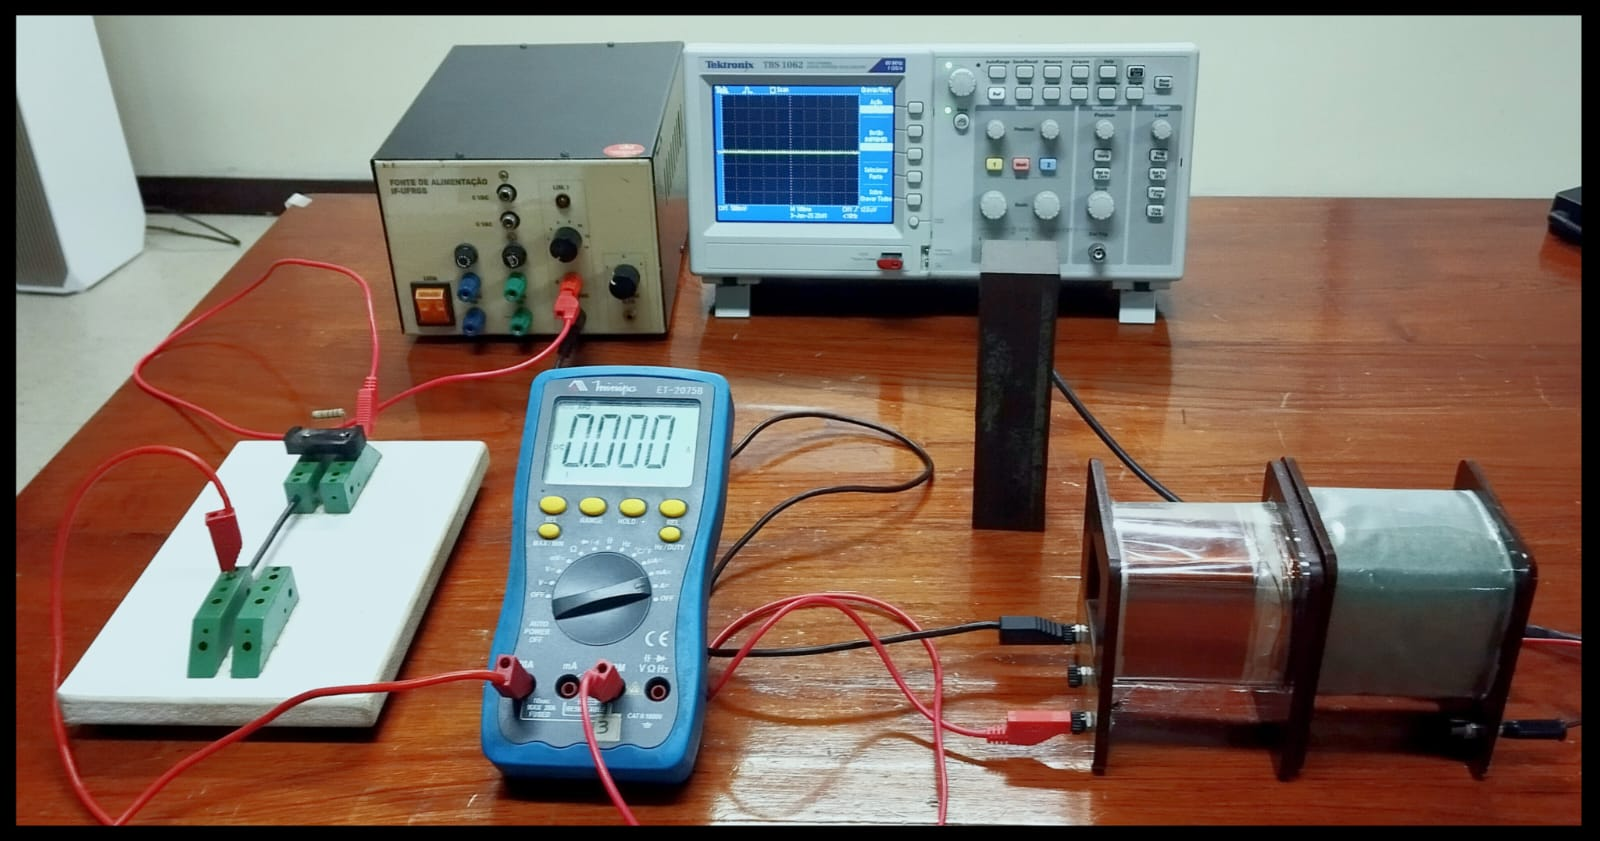
\includegraphics[width=1.04\linewidth]{Pasted image.png}
\captionof{figure}{Fonte, resistor, fios, multímetro, bobinas, núcleo de ferro e osciloscópio.}
    \label{fig:helmholtz-setup}
\end{minipage}
\newpage
\section{Procedimentos e Montagem}
\paragraph{}
Devemos, antes de tudo, separar as três montagens experimentais que serão estudadas neste relatório: em primeiro lugar, analisaremos a variação da tensão [V] induzida na bobina detectora (10.000 espiras) por um ímã natural; em segundo lugar, o mesmo para uma bobina geradora (1.000 espiras) juntamente à bobina detectora (10.000 espiras) e, por fim, para ambas as bobinas acrescidas de um núcleo metálico. 

\subsection{Montagem I}
\paragraph{}
\begin{itemize}
\item Conecte o osciloscópio aos terminais da bobina detectora diretamente.\\

\item Realize os ajustes necessários no equipamento para o salvamento de dados.\\
\end{itemize}

Tendo estruturado o sistema dessa maneira, manualmente insira o ímã no interior da bobina detectora. Busque posicioná-lo de tal forma que a remoção do ímã gere uma curva ascendente no gráfico e, quantas vezes se queira medir, salve a representação gráfica e os dados referentes a variação de tensão [V] na bobina ao remover o ímã manualmente. 

\subsection{Montagem II}
\begin{itemize}
\item Conecte a fonte de corrente ao resistor utilizando os fios.\\

\item Continue o circuito passando pelo multímetro em função de amperímetro.\\

\item Conecte o circuito à bobina geradora.\\

\item Feche o circuito de volta à fonte de corrente.\\

\item Separadamente conecte o osciloscópio à bobina detectora.\\

\item Encoste a bobina detectora à bobina geradora alinhando seus eixos.\\
\end{itemize}

Dessa vez, não utilize um ímã natural, mas sim a própria bobina geradora como eletroímã. Após alinhadas as bobinas, manualmente afaste a bobina detectora do eletroímã de forma rápida e meça  a variação de tensão [V]. Esse processo deverá ser repetido até que se tenha salvo uma quantidade satisfatória de medidas.

\subsection{Montagem III}

\begin{itemize}
\item Conecte a fonte de corrente ao resistor utilizando os fios.\\

\item Continue o circuito passando pelo multímetro em função de amperímetro.\\

\item Conecte o circuito à bobina geradora.\\

\item Feche o circuito de volta à fonte de corrente.\\

\item Separadamente conecte o osciloscópio à bobina detectora.\\ 

\item Insira o núcleo de ferro na bobina geradora buscando preencher todo seu interior.\\

\item Encoste a bobina detectora à bobina geradora alinhando seus eixos.\\
\end{itemize}

Por fim, realizaremos um processo semelhante àquele explicitado em 4.2, a diferença se fará pela presença do núcleo de ferro no interior do sistema que gerará alterações notáveis na variação de tensão [V] medida. Novamente, afaste a bobina detectora rapidamente e salve os dados coletados quantas vezes se queira.

\section{Dados Experimentais}
\paragraph{}
Os dados de tensão [$V$] em função do tempo [$s$] foram adquiridos com o auxílio de um osciloscópio como descrito na seção de procedimentos e montagem experimental. Para garantir a reprodutibilidade e avaliar a consistência dos resultados, registramos pelo menos 10 medições para cada um dos três cenários experimentais definidos: com a bobina geradora e o ímã, com a bobina geradora e a bobina detectora, sem o núcleo de ferro na geradora e por último com a bobina geradora e a bobina detectora, com a inserção do núcleo de ferro na geradora.

Os dados sobre as bobinas e suas dimensões são: 
\begin{table}[!htb]
    \centering
    \begin{tabular}{|c|c|}
        \hline
        Parâmetro & Valor \\
        \hline
        Número de espiras da bobina geradora & 1.000 \\
        Número de espiras da bobina detectora & 10.000 \\
        Comprimento das bobinas & $7,00.10^{-2} $m \\
        Área da seção transversal das bobinas & $2,5.10^{-3}$ m$^2$ \\
        \hline
    \end{tabular}
    \caption{Dados das bobinas utilizadas no experimento.}
    \label{tab:bobinas_dados}
\end{table}\\

A seguir, apresentamos um gráfico representativo de cada cenário. Para facilitar a visualização do evento de indução, os gráficos foram plotados no intervalo de tempo específico onde o pulso de tensão ocorre. A análise quantitativa subsequente focará na determinação do fluxo a partir da integral da curva V(t). O conjunto completo de dados em forma de gráficos para todas as medições pode ser consultado no apêndice ao final do relatório.

\begin{figure}[!htb]
    \centering
    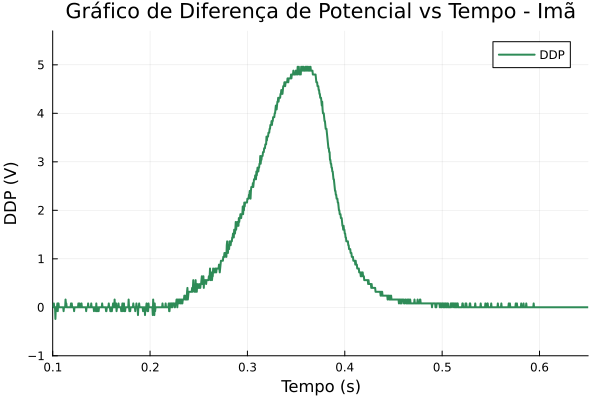
\includegraphics[width=0.6\textwidth]{figuras/grafico_diferenca_potencial - 1.png}
    \caption{Gráfico de tensão versus tempo com a bobina geradora e o imã.}
    \label{fig:grafico1}
\end{figure}
\begin{figure}[!htb]
    \centering
    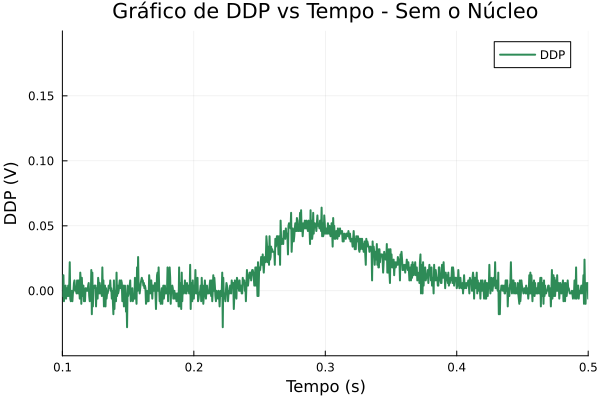
\includegraphics[width=0.6\textwidth]{figuras/grafico_diferenca_potencial - 2.png}
    \caption{Gráfico de tensão versus tempo com a bobina geradora e o detector sem o núcleo de ferro.}
    \label{fig:grafico2}
\end{figure}
\begin{figure}[!htb]
    \centering
    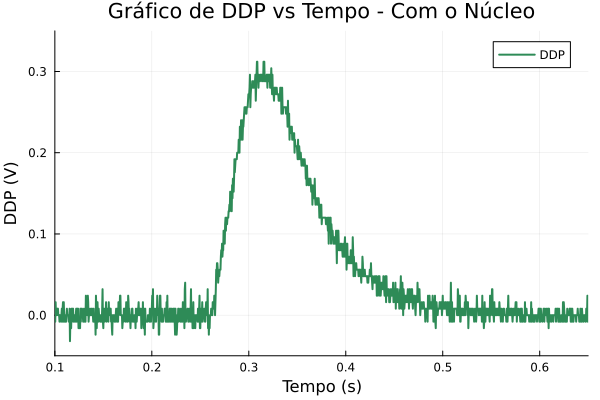
\includegraphics[width=0.6\textwidth]{figuras/grafico_diferenca_potencial - 3.png}
    \caption{Gráfico de tensão versus tempo com a bobina geradora e o detector com o núcleo de ferro.}
    \label{fig:grafico3}
\end{figure}
\newpage

\section{Análise de Dados}
\paragraph{}
De posse dos dados experimentais, utilizamos a integração numérica pelo método do trapézio para analisar a relação entre a tensão induzida e o fluxo magnético. Uma vez que os dados salvos do osciloscópio são em formato CSV, contendo todos os pontos do gráfico adquirido, usamos um programa em Julia para a integração numérica, o código está referenciado ao final do relatório.\\  
Conforme a Lei de Faraday, mais especificamente utilizando a relação expressa na equação (14), a integral da tensão em função do tempo está diretamente ligada à variação total do fluxo magnético através da bobina detectora. O resultado esperado é que o valor desta integral, $\int V(t)dt$, seja constante para todas as medições realizadas sob o mesmo cenário experimental. A justificativa para essa constância é que a variação total do fluxo magnético depende apenas das configurações inicial e final do sistema, que são as mesmas em cada repetição do experimento. As pequenas flutuações observadas entre os valores medidos são atribuídas às incertezas experimentais do procedimento.\\

Os resultados obtidos para o fluxo magnético e campo magnético são apresentados na tabela a seguir. A tabela inclui os valores médios e os desvios padrão, calculados a partir das medições realizadas.
\begin{table}[H]
    \centering
    \begin{tabular}{|c|c|c|c|}
        \hline
        Gerador do Campo $B$ & Fluxo Magnético ($\Phi$) & Desvio Padrão ($\sigma$)& Campo Magnético ($B$) \\
        \hline
        Ímã & $9,58.10^{-5}$ Wb &  $3,89.10^{-7}$ & $3,83.10^{-2}$ T \\
        Eletroimã - Sem Núcleo & $2,71.10^{-8}$ Wb & $9,34.10^{-10}$ & $1,08.10^{-5}$ T \\
        Eletroimã - Núcleo Fe & $5,60.10^{-7}$ Wb & $1,65.10^{-8}$ & $2,24.10^{-4}$ T \\
        \hline
    \end{tabular}
    \caption{Resultados dos fluxos magnéticos e campos magnéticos para os diferentes cenários experimentais.}
    \label{tab:resultados_fluxo_campo}
\end{table}
O desvio padrão observado nos valores de fluxo magnético é bastante baixo, indicando uma boa consistência entre as medições, conforme o esperado.
Usando os valores encontrados, e a propagação de incertezas, obtemos um valor para a constante de permeabilidade magnética do material do núcleo de ferro, $\mu$, que é calculada pela relação $\mu = \frac{B_{Nucleo}}{B_{Sem Nucleo}} . \mu_0$, igual a:
\begin{equation}
    2,60.10^{-5} \pm 4,71.10^{-7} \frac{T.m}{A}. 
\end{equation}
Esse valor é plausível, pois está na ordem de grandeza esperada para materiais compostos de ferro com impurezas.

\section{Conclusão}
\paragraph{}
Após realizada a análise numérica dos dados coletados, podemos dissertar sobre o quão bem as relações teóricas se expressaram em nosso experimento, levando em consideração as incertezas tanto numéricas quanto as inerentes ao método experimental utilizado: nosso primeiro objetivo consistiu-se da verificação da constância esperada no valor das áreas sobre as curvas de tensão [V]. Como citado na sessão \textbf{Análise de Dados}, o método do trapézio foi utilizado para a integração dos dados coletados e, por meio de análise estatística, verificamos que o desvio padrão ($\sigma$) existente nos valores de fluxo magnético ($\Phi$) advindos dessas medidas tem quantia máxima de $3,89.10^{-7}$. Isso significa que a maior diferença entre as áreas de tensão [V] em função de tempo [s] está na ordem de grandeza $10^{-7}$, um número extremamente baixo que explicita constância satisfatória entre as áreas.

Ademais, para determinarmos a constante de permeabilidade magnética ($\mu$)
do núcleo de ferro utilizado na montagem III e os campos magnéticos (B) necessários para tal, as equações deduzidas na sessão \textbf{Embasamento Teórico} foram utilizadas juntamente com os dados calculados referentes ao fluxo magnético ($\Phi$), entregando-nos um campo magnético de maior valor para a montagem I, com o campo de II vindo atrás de ambos os demais. O fato do campo em III ser maior do que em II concorda com o valor de ($\mu$) obtido para o núcleo de ferro: $2,60.10^{-5} \pm 4,71.10^{^-7} \frac{T.m}{A}$. Este valor é maior do que o valor referente a permeabilidade magnética do vácuo, $4\pi.10^{-7}\frac{T.m}{A}$, de tal forma que, segundo (10), resultaria, de fato, num campo magnético (B) maior para a montagem III (com a presença do núcleo). 

Pois, o experimento se mostrou suficiente em possibilitar o estudo e análise das relações existentes entre a eletricidade e o magnetismo. Os valores obtidos para tensão, os fluxos e campos calculados assim como a permeabilidade do núcleo ferroso se encaixam dentro um padrão esperado e tem sentido coerente com a premissa teórica, até mesmo as incertezas se mostraram relativamente pequenas tanto para a constante magnética como para a diferença entre as áreas dos gráficos de tensão em função do tempo. Isso dito, podemos sugerir apenas que experimentos futuros busquem materiais ainda mais puros para o núcleo e posterior análise assim como a busca de equipamentos que permitam um manuseio mais preciso do ímã e da bobina detectora com uma melhor reprodutibilidade.


\begin{thebibliography}{99}

\bibitem{}
Processamento de dados e produção de gráficos:
\url{https://github.com/pedro-hro/Relatorio_6-ExperimentalIII}
\bibitem{}
RUTH W. CHABBAY. Matter and Interactions 4th Edition - Matter and Interactions, 4th Edition. WILEY, 2015.
\bibitem{}
NUSSENZVEIG, H. Moysés. {\em Curso de Física Básica - Mecânica}. 5ª ed., vol. 3. São Paulo: Edgard Blücher Ltda, 2013.
\bibitem{}
MAGNETIC FIELD OF A SOLENOID. Magnetic Field of a Solenoid -
        Student Handout - 04-magnetic-field-solenoid.pdf.
        Disponível em: \url{http://physics.wku.edu/harper/files/apps/pla/examples/04-magnetic-field-solenoid.pdf}. Acesso em: 4 de Junho de 2025.

\end{thebibliography}

%\section*{Apêndice - Gráficos de DDP vs Tempo}
\section*{Gráficos de DDP vs Tempo}
\begin{center}
\begin{multicols}{2}

\begin{figure}[H]
    \centering
    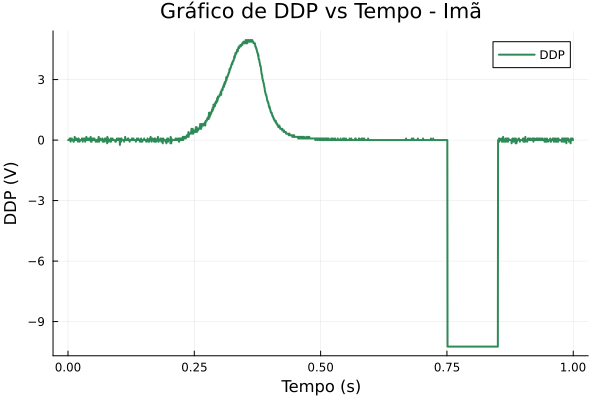
\includegraphics[width=1.0\linewidth]{figuras/grafico_dados1_F0002CH1.png}
\end{figure}

\begin{figure}[H]
    \centering
    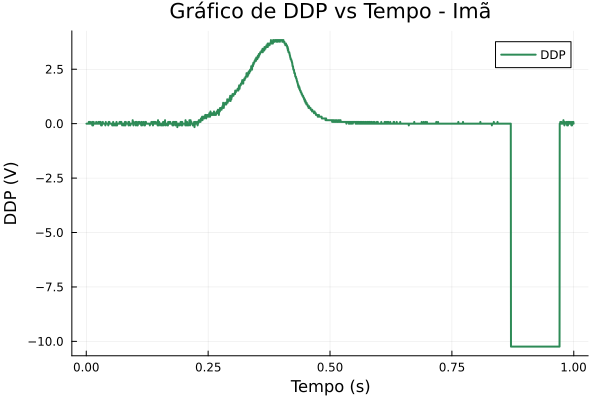
\includegraphics[width=1.0\linewidth]{figuras/grafico_dados1_F0003CH1.png}
\end{figure}

\begin{figure}[H]
    \centering
    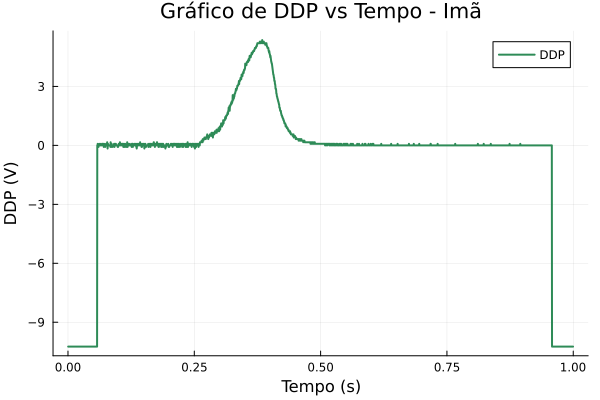
\includegraphics[width=1.0\linewidth]{figuras/grafico_dados1_F0004CH1.png}
\end{figure}

\begin{figure}[H]
    \centering
    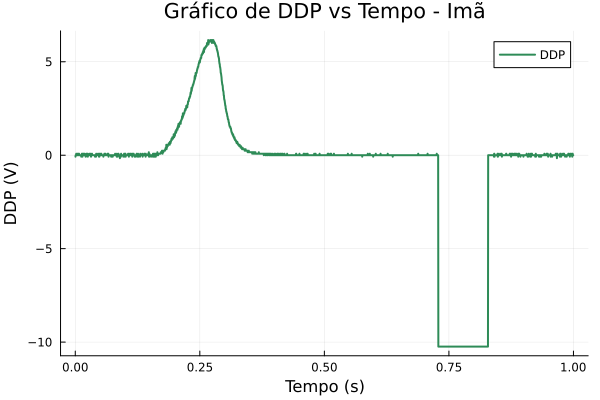
\includegraphics[width=1.0\linewidth]{figuras/grafico_dados1_F0005CH1.png}
\end{figure}

\begin{figure}[H]
    \centering
    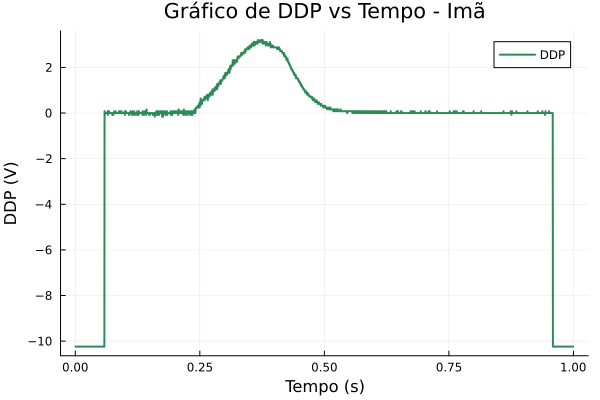
\includegraphics[width=1.0\linewidth]{figuras/grafico_dados1_F0006CH1.png}
\end{figure}

\begin{figure}[H]
    \centering
    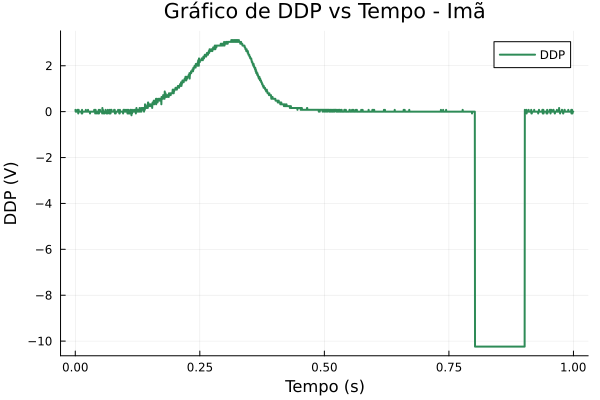
\includegraphics[width=1.0\linewidth]{figuras/grafico_dados1_F0007CH1.png}
\end{figure}

\begin{figure}[H]
    \centering
    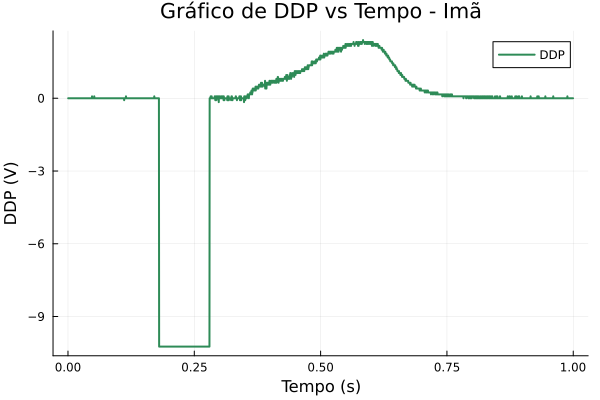
\includegraphics[width=1.0\linewidth]{figuras/grafico_dados1_F0008CH1.png}
\end{figure}

\begin{figure}[H]
    \centering
    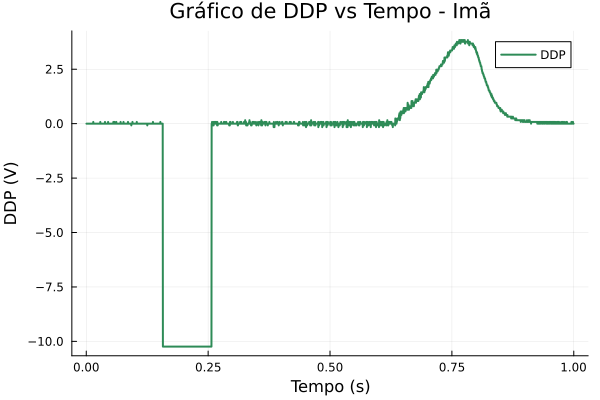
\includegraphics[width=1.0\linewidth]{figuras/grafico_dados1_F0009CH1.png}
\end{figure}

\begin{figure}[H]
    \centering
    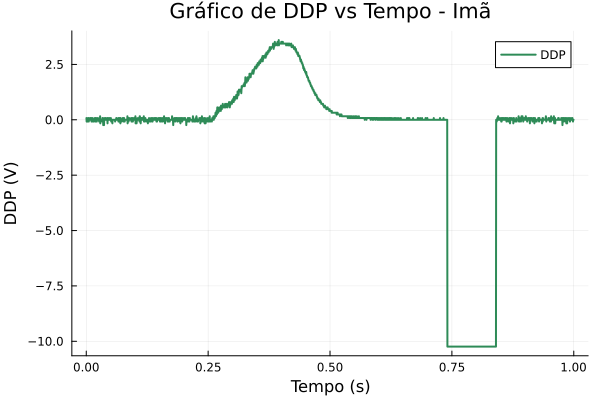
\includegraphics[width=1.0\linewidth]{figuras/grafico_dados1_F0010CH1.png}
\end{figure}

\begin{figure}[H]
    \centering
    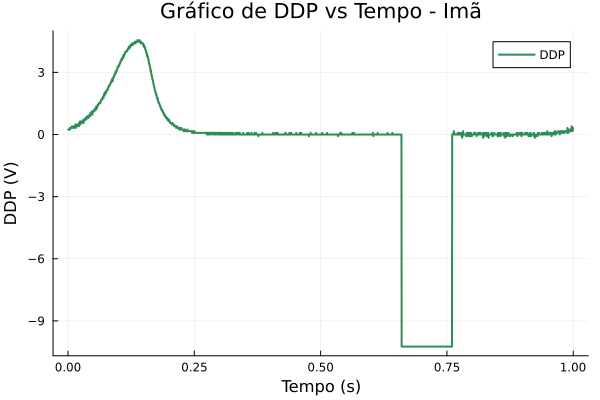
\includegraphics[width=1.0\linewidth]{figuras/grafico_dados1_F0011CH1.png}
\end{figure}

\begin{figure}[H]
    \centering
    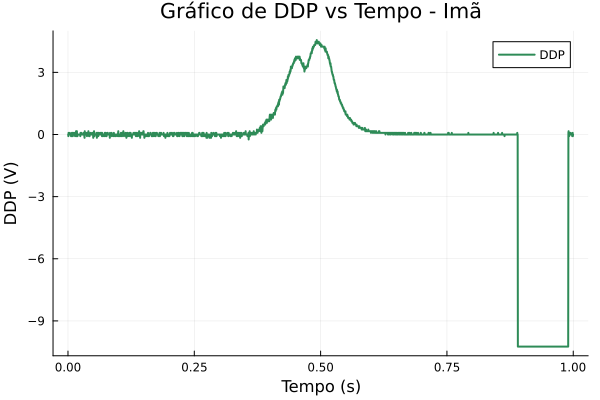
\includegraphics[width=1.0\linewidth]{figuras/grafico_dados1_F0012CH1.png}
\end{figure}

\begin{figure}[H]
    \centering
    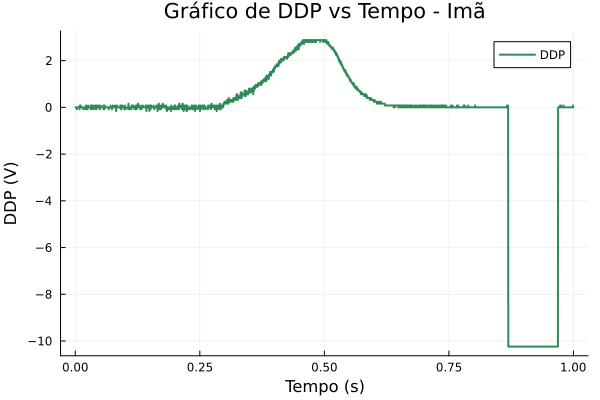
\includegraphics[width=1.0\linewidth]{figuras/grafico_dados1_F0013CH1.png}
\end{figure}

\begin{figure}[H]
    \centering
    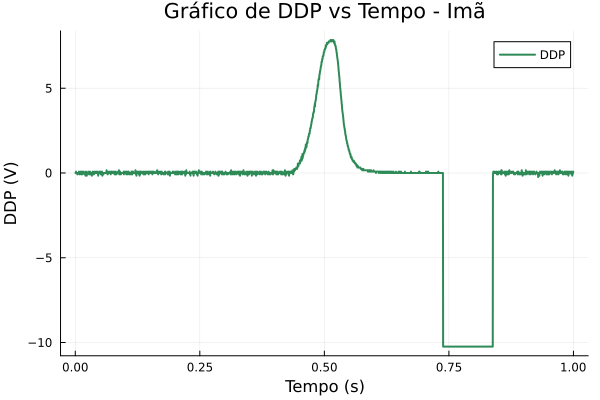
\includegraphics[width=1.0\linewidth]{figuras/grafico_dados1_F0014CH1.png}
\end{figure}

\begin{figure}[H]
    \centering
    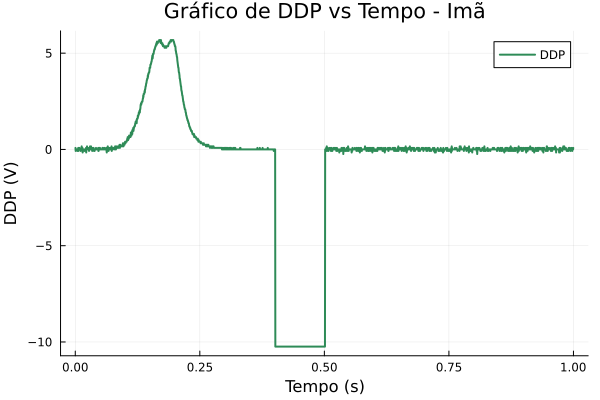
\includegraphics[width=1.0\linewidth]{figuras/grafico_dados1_F0016CH1.png}
\end{figure}

\begin{figure}[H]
    \centering
    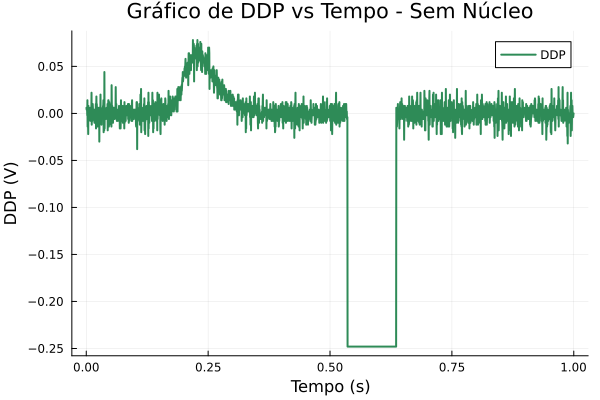
\includegraphics[width=1.0\linewidth]{figuras/grafico_dados2_F0000CH1.png}
\end{figure}

\begin{figure}[H]
    \centering
    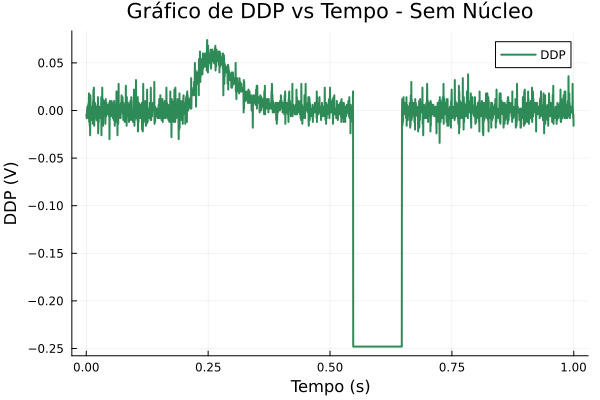
\includegraphics[width=1.0\linewidth]{figuras/grafico_dados2_F0001CH1.png}
\end{figure}

\begin{figure}[H]
    \centering
    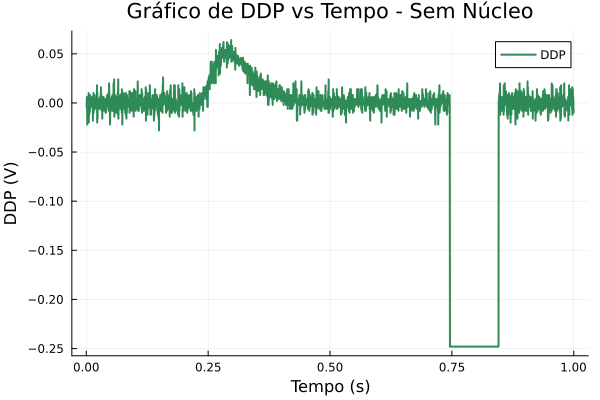
\includegraphics[width=1.0\linewidth]{figuras/grafico_dados2_F0002CH1.png}
\end{figure}

\begin{figure}[H]
    \centering
    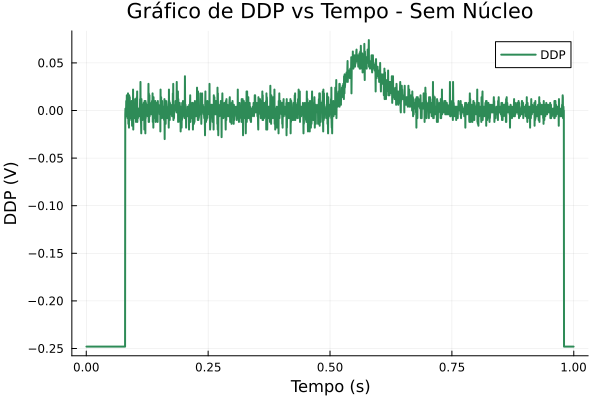
\includegraphics[width=1.0\linewidth]{figuras/grafico_dados2_F0003CH1.png}
\end{figure}

\begin{figure}[H]
    \centering
    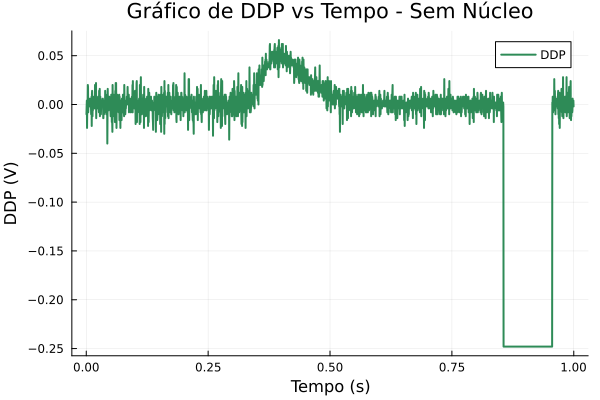
\includegraphics[width=1.0\linewidth]{figuras/grafico_dados2_F0004CH1.png}
\end{figure}

\begin{figure}[H]
    \centering
    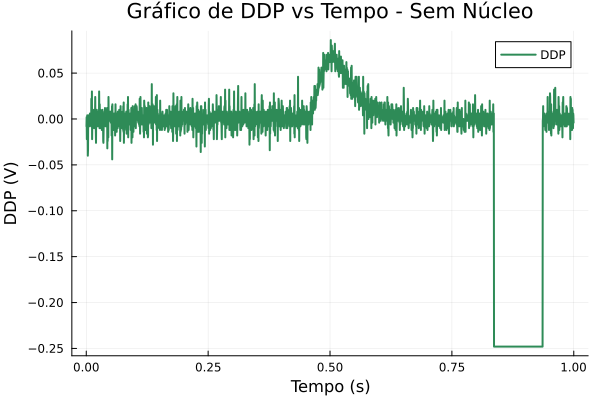
\includegraphics[width=1.0\linewidth]{figuras/grafico_dados2_F0005CH1.png}
\end{figure}

\begin{figure}[H]
    \centering
    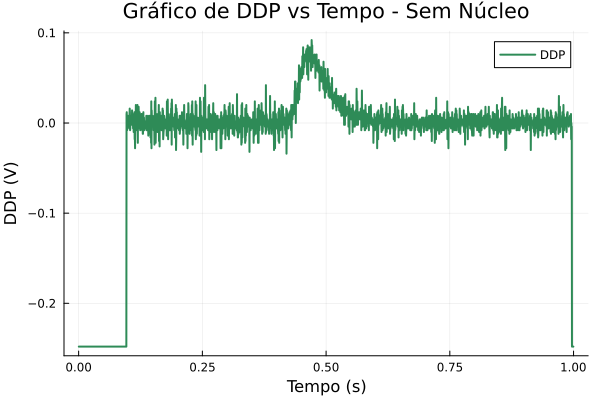
\includegraphics[width=1.0\linewidth]{figuras/grafico_dados2_F0006CH1.png}
\end{figure}

\begin{figure}[H]
    \centering
    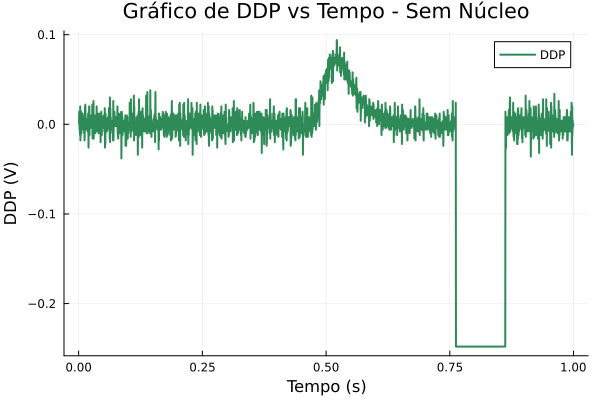
\includegraphics[width=1.0\linewidth]{figuras/grafico_dados2_F0007CH1.png}
\end{figure}

\begin{figure}[H]
    \centering
    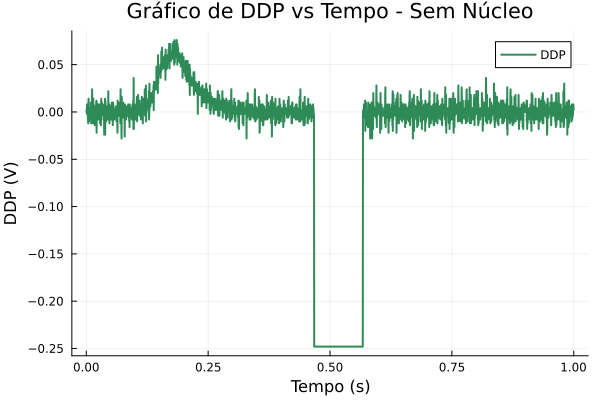
\includegraphics[width=1.0\linewidth]{figuras/grafico_dados2_F0008CH1.png}
\end{figure}

\begin{figure}[H]
    \centering
    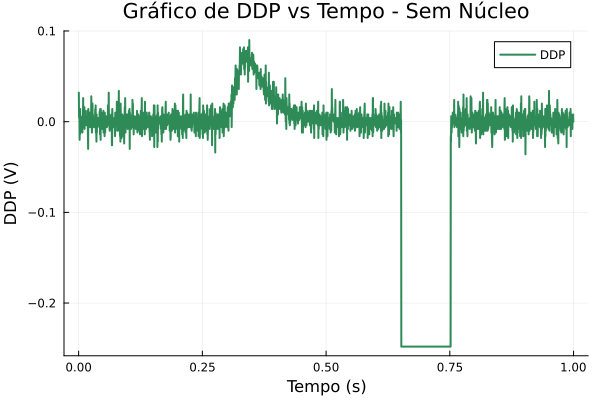
\includegraphics[width=1.0\linewidth]{figuras/grafico_dados2_F0009CH1.png}
\end{figure}

\begin{figure}[H]
    \centering
    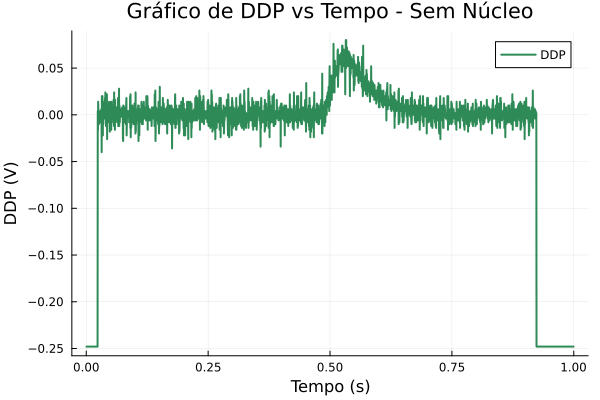
\includegraphics[width=1.0\linewidth]{figuras/grafico_dados2_F0010CH1.png}
\end{figure}

\begin{figure}[H]
    \centering
    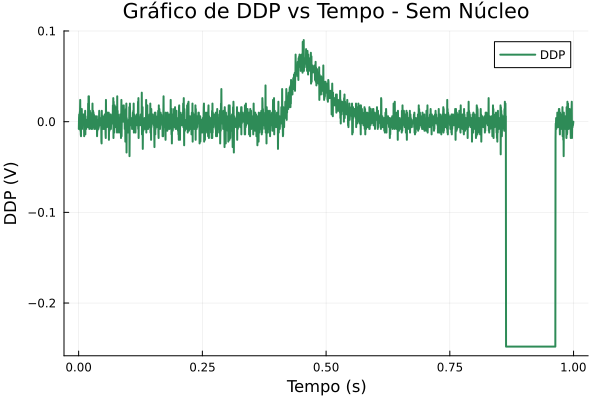
\includegraphics[width=1.0\linewidth]{figuras/grafico_dados2_F0011CH1.png}
\end{figure}

\begin{figure}[H]
    \centering
    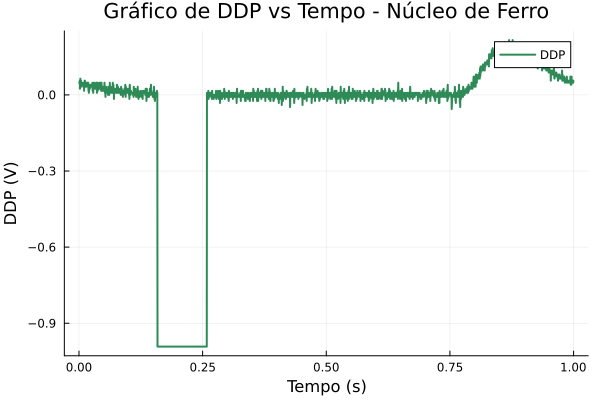
\includegraphics[width=1.0\linewidth]{figuras/grafico_dados3_F0000CH1.png}
\end{figure}

\begin{figure}[H]
    \centering
    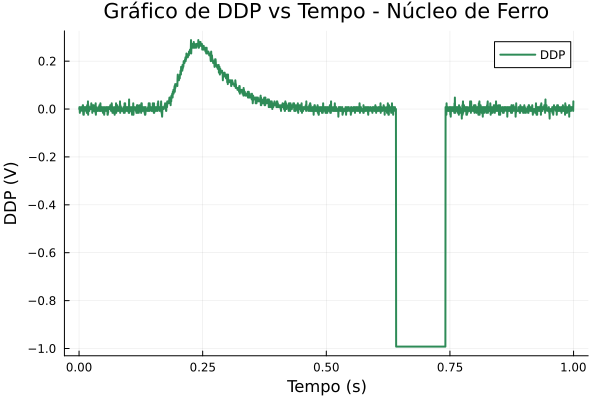
\includegraphics[width=1.0\linewidth]{figuras/grafico_dados3_F0001CH1.png}
\end{figure}

\begin{figure}[H]
    \centering
    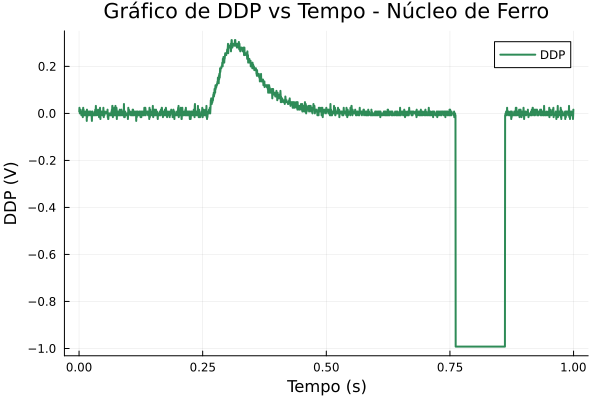
\includegraphics[width=1.0\linewidth]{figuras/grafico_dados3_F0002CH1.png}
\end{figure}

\begin{figure}[H]
    \centering
    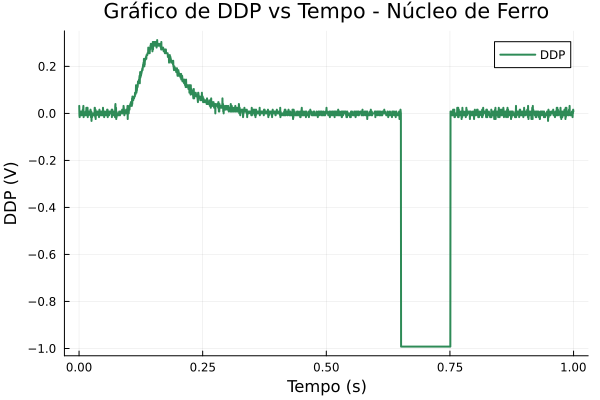
\includegraphics[width=1.0\linewidth]{figuras/grafico_dados3_F0003CH1.png}
\end{figure}

\begin{figure}[H]
    \centering
    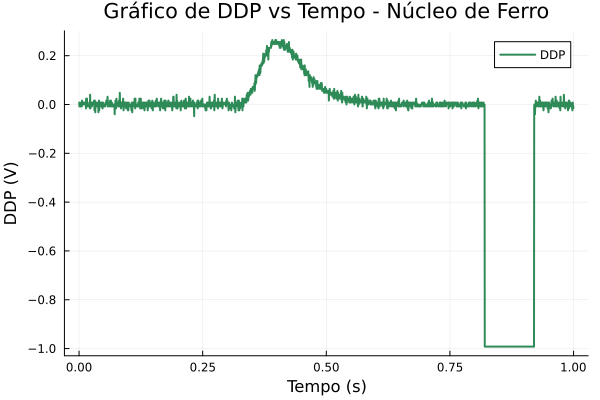
\includegraphics[width=1.0\linewidth]{figuras/grafico_dados3_F0004CH1.png}
\end{figure}

\begin{figure}[H]
    \centering
    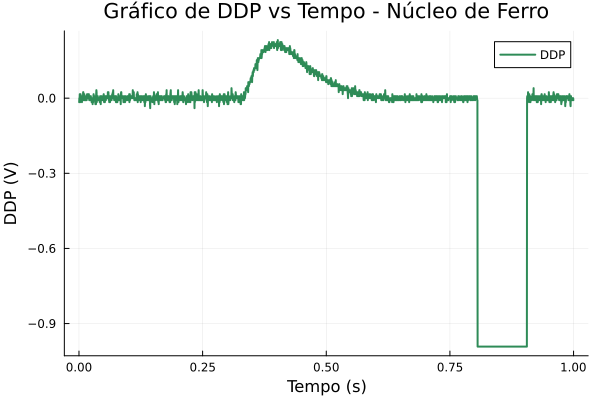
\includegraphics[width=1.0\linewidth]{figuras/grafico_dados3_F0005CH1.png}
\end{figure}

\begin{figure}[H]
    \centering
    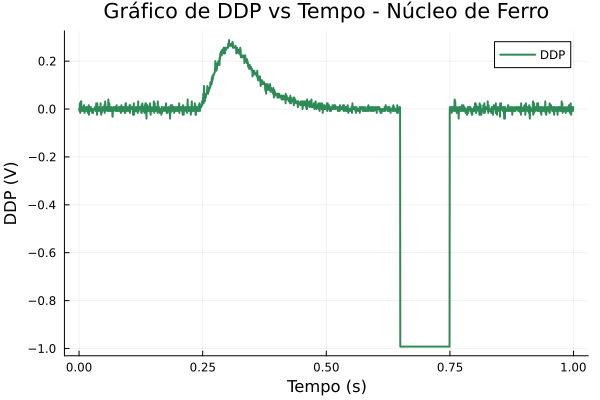
\includegraphics[width=1.0\linewidth]{figuras/grafico_dados3_F0006CH1.png}
\end{figure}

\begin{figure}[H]
    \centering
    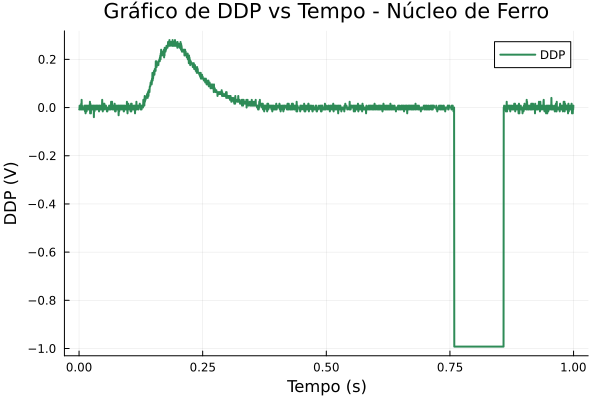
\includegraphics[width=1.0\linewidth]{figuras/grafico_dados3_F0007CH1.png}
\end{figure}

\begin{figure}[H]
    \centering
    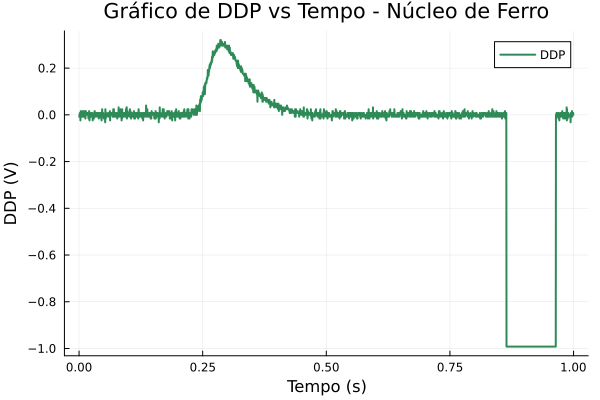
\includegraphics[width=1.0\linewidth]{figuras/grafico_dados3_F0008CH1.png}
\end{figure}

\begin{figure}[H]
    \centering
    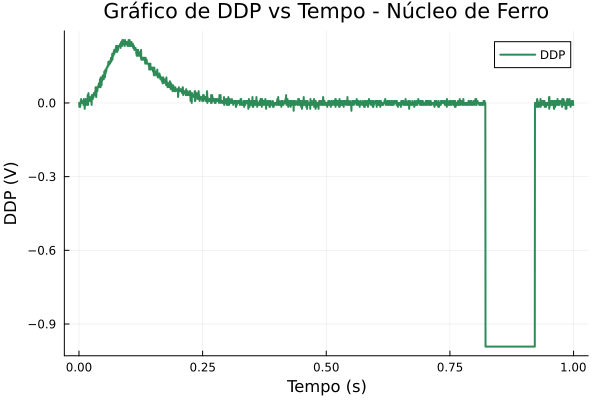
\includegraphics[width=1.0\linewidth]{figuras/grafico_dados3_F0009CH1.png}
\end{figure}

\begin{figure}[H]
    \centering
    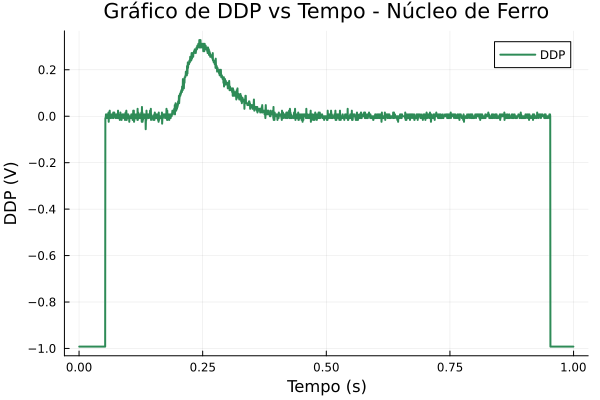
\includegraphics[width=1.0\linewidth]{figuras/grafico_dados3_F0010CH1.png}
\end{figure}

\begin{figure}[H]
    \centering
    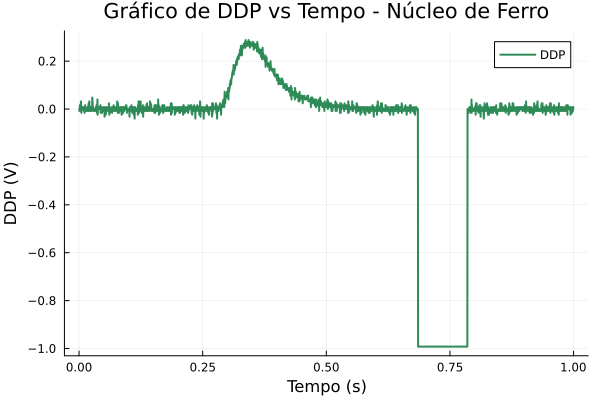
\includegraphics[width=1.0\linewidth]{figuras/grafico_dados3_F0011CH1.png}
\end{figure}

\begin{figure}[H]
    \centering
    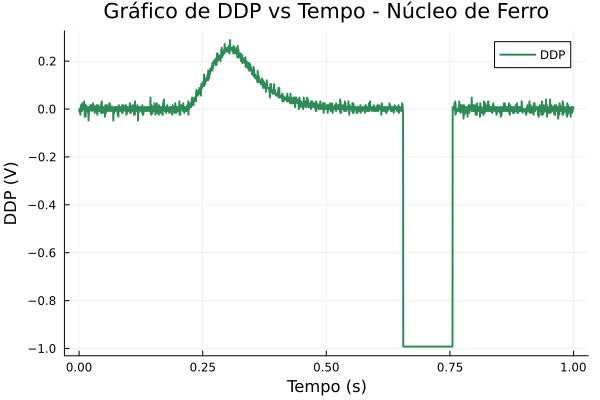
\includegraphics[width=1.0\linewidth]{figuras/grafico_dados3_F0012CH1.png}
\end{figure}

\end{multicols}
\end{center}



\end{document}